\documentclass[11pt]{article}
\usepackage[margin=0.85in]{geometry}
\usepackage{amsmath,amssymb,mathtools,enumitem,booktabs}
\usepackage[T1]{fontenc}
\usepackage{lmodern}
\usepackage{pgfplots}
\pgfplotsset{compat=1.18}
\usepackage[colorlinks=true,linkcolor=blue]{hyperref}
\newcommand{\ex}[1]{\subsection*{#1.}}
\newcommand{\ans}[1]{\boxed{#1}}
\newcommand{\vv}[1]{\left\langle #1\right\rangle}
\newcommand{\ii}{\mathbf i}\newcommand{\jj}{\mathbf j}\newcommand{\kk}{\mathbf k}
\newcommand{\cp}[6]{\begin{vmatrix}\ii&\jj&\kk\\#1&#2&#3\\#4&#5&#6\end{vmatrix}}
\pgfplotsset{every axis/.append style={width=.70\linewidth,height=6cm,xlabel={$x$},ylabel={$y$},zlabel={$z$},view={125}{25},grid=major}}
\newcommand{\surf}[4]{\begin{center}\begin{tikzpicture}\begin{axis}[#1]\addplot3[surf,shader=interp,samples=19,samples y=19,opacity=.78] ({#2},{#3},{#4});\end{axis}\end{tikzpicture}\end{center}}
\newcommand{\curve}[4]{\begin{center}\begin{tikzpicture}\begin{axis}[#1]\addplot3[blue,thick,samples=180,samples y=0,variable=t] ({#2},{#3},{#4});\end{axis}\end{tikzpicture}\end{center}}
\title{Chapter 15: Multiple Integrals\\Worked solutions to the assigned exercises}
\author{}\date{}\begin{document}\maketitle
\noindent Source: Stewart, Clegg, and Watson, ninth edition. This chapter follows the assignment screenshot. Each iterated integral is evaluated from the inside outward, holding the outside variable fixed during the inner integration.
\tableofcontents
\clearpage\section*{15.1 Double Integrals over Rectangles}\addcontentsline{toc}{section}{15.1 Double Integrals over Rectangles}
\ex{3}
The rectangle is $[0,2]\times[0,1]$ and $f=xe^{-xy}$. With $m=n=2$, $\Delta x=1$, $\Delta y=1/2$, and $\Delta A=1/2$.
\begin{enumerate}[label=(\alph*)]
\item The upper-right points are $(1,1/2),(1,1),(2,1/2),(2,1)$. Therefore
\[\iint_R f\,dA\approx\tfrac12[e^{-1/2}+e^{-1}+2e^{-1}+2e^{-2}]
=\ans{\tfrac12e^{-1/2}+\tfrac32e^{-1}+e^{-2}\approx .99042}.\]
\item The midpoints are $(1/2,1/4),(1/2,3/4),(3/2,1/4),(3/2,3/4)$. Thus
\[\iint_R f\,dA\approx\tfrac12[\tfrac12e^{-1/8}+\tfrac12e^{-3/8}+\tfrac32e^{-3/8}+\tfrac32e^{-9/8}]
=\ans{\tfrac14e^{-1/8}+e^{-3/8}+\tfrac34e^{-9/8}\approx1.15140}.\]
These are estimates from four samples, not exact values of the integral.
\end{enumerate}
\ex{5}
For $f=\sqrt{52-x^2-y^2}$ on $2\le x\le4$, $2\le y\le6$, increasing either positive coordinate decreases the radicand and hence decreases $f$. In every subrectangle, the lower-left corner has the largest height and the upper-right has the smallest. Therefore $L$ is an upper bound on the actual volume and $U$ a lower bound:
\[\ans{U<V<L}.\]
The inequalities are strict because the surface is not constant on any positive-area subrectangle. The letters describe corner locations, not lower and upper numerical bounds.
\ex{7}
\begin{enumerate}[label=(\alph*)]
\item Dividing $[0,4]^2$ into four squares gives $\Delta A=4$ and midpoints $(1,1),(3,1),(1,3),(3,3)$. Reading the contour map gives approximate heights $25,25,0,15$, respectively. The first two lie between levels $20$ and $30$, the third is near the zero contour, and the fourth between $10$ and $20$. Hence
\[\ans{\iint_R f\,dA\approx4(25+25+0+15)=260}.\]
\item The rectangle area is $16$. Thus $\ans{f_{\mathrm{avg}}\approx260/16=16.25}$. Small differences in visual readings are expected; the map does not specify exact midpoint values.
\end{enumerate}
\ex{9}
The constant height $\sqrt2$ over $2\le x\le6$, $-1\le y\le5$ forms a rectangular prism. Its base area is $(6-2)(5-(-1))=24$. Thus its volume, and the integral, is $\ans{24\sqrt2}$.
\ex{11}
The height $4-2y$ decreases from $4$ to $2$ as $y$ runs from $0$ to $1$, independent of $x\in[0,1]$. The solid is a prism with a trapezoidal cross-section of area $\tfrac12(4+2)(1)=3$ and length $1$. Hence $\ans{\iint_R(4-2y)\,dA=3}$.
\ex{13}
For $f=x+3x^2y^2$, first integrate in $x$, treating $y$ as constant:
\[\ans{\int_0^2f(x,y)\,dx=\left[\frac{x^2}{2}+x^3y^2\right]_0^2=2+8y^2}.\]
Then, separately, integrate in $y$, treating $x$ as constant:
\[\ans{\int_0^3f(x,y)\,dy=[xy+x^2y^3]_0^3=3x+27x^2}.\]
These are functions of the remaining variable, not double integrals.
\ex{15}
\begin{align*}
\int_1^4\int_0^2(6x^2y-2x)\,dy\,dx
&=\int_1^4[3x^2y^2-2xy]_0^2\,dx\\
&=\int_1^4(12x^2-4x)\,dx=[4x^3-2x^2]_1^4\\
&=(256-32)-(4-2)=\ans{222}.
\end{align*}
\ex{19}
\begin{align*}
\int_{-3}^3\int_0^{\pi/2}(y+y^2\cos x)\,dx\,dy
&=\int_{-3}^3[xy+y^2\sin x]_0^{\pi/2}\,dy\\
&=\int_{-3}^3\left(\frac\pi2y+y^2\right)dy
=\left[\frac\pi4y^2+\frac{y^3}{3}\right]_{-3}^3=\ans{18}.
\end{align*}
The odd linear term cancels over the symmetric interval.
\ex{21}
\begin{align*}
\int_1^4\int_1^2\left(\frac xy+\frac yx\right)dy\,dx
&=\int_1^4\left[x\ln y+\frac{y^2}{2x}\right]_1^2dx\\
&=\int_1^4\left(x\ln2+\frac3{2x}\right)dx\\
&=\left[\frac{x^2}{2}\ln2+\frac32\ln x\right]_1^4
=\frac{15}2\ln2+\frac32\ln4=\ans{\frac{21}2\ln2}.
\end{align*}
\ex{25}
Integrate first in $u$ using the power rule, since $v$ is constant:
\begin{align*}
\int_0^1\int_0^1v(u+v^2)^4\,du\,dv
&=\frac15\int_0^1v[(1+v^2)^5-v^{10}]\,dv\\
&=\frac15\left[\frac{(1+v^2)^6}{12}-\frac{v^{12}}{12}\right]_0^1\\
&=\frac{64-1-1}{60}=\ans{\frac{31}{30}}.
\end{align*}
The antiderivative of $v(1+v^2)^5$ uses $q=1+v^2$, $dq=2v\,dv$.
\ex{27}
Over $0\le x\le2$, $0\le y\le\pi/4$,
\[\iint_R x\sec^2y\,dA=\int_0^2[x\tan y]_0^{\pi/4}\,dx
=\int_0^2x\,dx=[x^2/2]_0^2=\ans{2}.\]
\ex{29}
\begin{align*}
\iint_R\frac{xy^2}{x^2+1}\,dA
&=\int_0^1\frac{x}{x^2+1}\left[\frac{y^3}{3}\right]_{-3}^3dx\\
&=18\int_0^1\frac{x}{x^2+1}dx
=9[\ln(x^2+1)]_0^1=\ans{9\ln2}.
\end{align*}
Here $q=x^2+1$, $dq=2x\,dx$ accounts for the factor $1/2$.
\ex{31}
\begin{align*}
I&=\int_0^{\pi/6}\int_0^{\pi/3}x\sin(x+y)\,dy\,dx\\
&=\int_0^{\pi/6}x[\cos x-\cos(x+\pi/3)]\,dx.
\end{align*}
Integration by parts gives $\int x\cos(x+c)dx=x\sin(x+c)+\cos(x+c)$ (choose $u=x$, $dv=\cos(x+c)dx$). Therefore
\begin{align*}
I&=[x\sin x+\cos x-x\sin(x+\pi/3)-\cos(x+\pi/3)]_0^{\pi/6}\\
&=\left(\frac\pi{12}+\frac{\sqrt3}{2}-\frac\pi6-0\right)-(1-1/2)
=\ans{\frac{\sqrt3-1}{2}-\frac\pi{12}}.
\end{align*}
\ex{35}
The solid has $0\le x,y\le1$ and $0\le z\le4-x-2y$. Its top is a plane with heights $4,3,2,1$ over the four corners $(0,0),(1,0),(0,1),(1,1)$. Its vertical side faces lie in $x=0,1$, $y=0,1$, and its bottom is $z=0$.
\begin{center}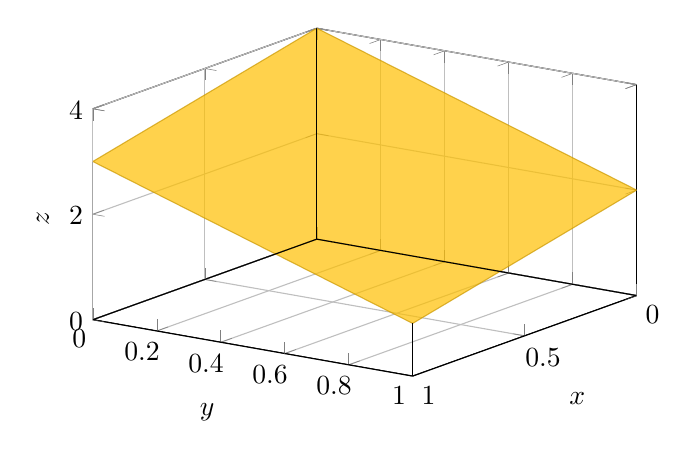
\begin{tikzpicture}\begin{axis}[domain=0:1,y domain=0:1,zmin=0,zmax=4]\addplot3[surf,opacity=.7,samples=2]{4-x-2*y};\addplot3[black] coordinates {(0,0,0)(1,0,0)(1,1,0)(0,1,0)(0,0,0)};\addplot3[black] coordinates {(0,0,0)(0,0,4)};\addplot3[black] coordinates {(1,0,0)(1,0,3)};\addplot3[black] coordinates {(1,1,0)(1,1,1)};\addplot3[black] coordinates {(0,1,0)(0,1,2)};\end{axis}\end{tikzpicture}\end{center}
\ex{42}
\begin{enumerate}[label=(\alph*)]
\item The figure shows $z=x^2+y^2$ over $0\le x\le2$, $0\le y\le3$. Thus $\ans{V=\int_0^2\int_0^3(x^2+y^2)\,dy\,dx}$.
\item Evaluate: $\int_0^3(x^2+y^2)dy=[x^2y+y^3/3]_0^3=3x^2+9$. Then $V=[x^3+9x]_0^2=8+18=\ans{26}$.
\end{enumerate}
\ex{49}
The top is $z=2+x^2+(y-2)^2$ and the bottom is $z=1$ on $-1\le x\le1$, $0\le y\le4$. The height is therefore $1+x^2+(y-2)^2$, everywhere positive:
\begin{align*}
V&=\int_{-1}^1\int_0^4[1+x^2+(y-2)^2]dy\,dx\\
&=\int_{-1}^1\left[4(1+x^2)+\frac{(y-2)^3}{3}\bigg|_0^4\right]dx\\
&=\int_{-1}^1\left(\frac{28}3+4x^2\right)dx
=\frac{56}3+\frac83=\ans{\frac{64}3}.
\end{align*}
\clearpage\section*{15.2 Double Integrals over General Regions}\addcontentsline{toc}{section}{15.2 Double Integrals over General Regions}
\ex{1}
\[\int_1^5\int_0^x(8x-2y)dy\,dx=\int_1^5[8xy-y^2]_0^x dx
=7\int_1^5x^2dx=\frac73(125-1)=\ans{868/3}.\]
\ex{3}
Since $e^{y^3}$ is constant in the inner integral,
\[\int_0^1\int_0^yxe^{y^3}dx\,dy=\frac12\int_0^1y^2e^{y^3}dy
=\frac16[e^{y^3}]_0^1=\ans{(e-1)/6}.\]
The substitution $u=y^3$, $du=3y^2dy$ gives the outside antiderivative.
\ex{5}
\[\int_0^1\int_0^{s^2}\cos(s^3)dt\,ds=\int_0^1s^2\cos(s^3)ds
=\frac13[\sin(s^3)]_0^1=\ans{\sin1/3}.\]
Here $u=s^3$, $du=3s^2ds$.
\ex{7}
\begin{enumerate}[label=(\alph*)]
\item Intersections of $y=x$ and $y=3x-x^2$ satisfy $x(2-x)=0$, so $0\le x\le2$, with the line below the parabola. Hence $\ans{I=\int_0^2\int_x^{3x-x^2}2y\,dy\,dx}$.
\item $I=\int_0^2[(3x-x^2)^2-x^2]dx=\int_0^2(8x^2-6x^3+x^4)dx$. Therefore $I=[8x^3/3-3x^4/2+x^5/5]_0^2=64/3-24+32/5=\ans{56/15}$.
\end{enumerate}
\ex{9}
\begin{enumerate}[label=(\alph*)]
\item The shaded region has $0\le y\le2$, bounded on the left by $x=y^2$ and on the right by $x=y+2$. The height variable $y$ ends at $2$ because $y^2=y+2$ has nonnegative root $2$. Thus $\ans{I=\int_0^2\int_{y^2}^{y+2}xy\,dx\,dy}$.
\item Integrating in $x$ gives $I=\frac12\int_0^2y[(y+2)^2-y^4]dy$. Expand and integrate:
\[I=\left[\frac{y^4}{8}+\frac{2y^3}{3}+y^2-\frac{y^6}{12}\right]_0^2
=2+16/3+4-16/3=\ans{6}.\]
\end{enumerate}
\ex{17}
\begin{enumerate}[label=(\alph*)]
\item Type I: $0\le x\le1$, $0\le y\le x$. Hence $I=\int_0^1\int_0^x x\,dy\,dx=\int_0^1x^2dx=\ans{1/3}$.
\item Type II: $0\le y\le1$, $y\le x\le1$. Hence $I=\int_0^1\int_y^1x\,dx\,dy=\frac12\int_0^1(1-y^2)dy=\ans{1/3}$.
\end{enumerate}
Both describe the same triangle below $y=x$ in the unit square, so they must agree.
\ex{19}
Intersect $x=y^2$ and $x=y+2$: $y^2-y-2=(y-2)(y+1)=0$, giving $y=-1,2$. The easier order is
\[I=\int_{-1}^2\int_{y^2}^{y+2}y\,dx\,dy.\]
For the other order, vertical slices change their lower boundary at $x=1$:
\[I=\int_0^1\int_{-\sqrt x}^{\sqrt x}y\,dy\,dx+\int_1^4\int_{x-2}^{\sqrt x}y\,dy\,dx.\]
Using the first order avoids splitting:
\[I=\int_{-1}^2y(y+2-y^2)dy=[-y^4/4+y^3/3+y^2]_{-1}^2
=8/3-5/12=\ans{9/4}.\]
\ex{21}
The two orders are
\[I=\int_0^{\pi/2}\int_0^{\cos x}\sin^2x\,dy\,dx
=\int_0^1\int_0^{\arccos y}\sin^2x\,dx\,dy.\]
The first is easier: the inside integration just multiplies by $\cos x$, providing a substitution for the outside integral:
\[I=\int_0^{\pi/2}\sin^2x\cos x\,dx=\int_0^1u^2du=[u^3/3]_0^1=\ans{1/3},\quad u=\sin x.\]
\ex{23}
The region has $0\le x\le1$, $0\le y\le x^2$:
\[I=\int_0^1\int_0^{x^2}x\cos y\,dy\,dx=\int_0^1x\sin(x^2)dx.
\]
With $u=x^2$, $du=2x\,dx$, $I=\frac12\int_0^1\sin u\,du=\ans{(1-\cos1)/2}$.
\ex{25}
Horizontal slices of the triangle with vertices $(0,1),(1,2),(4,1)$ run from $x=y-1$ to $x=7-3y$, for $1\le y\le2$. These equations follow from the lines through the upper vertex and the respective lower vertices. Thus
\[I=\int_1^2\int_{y-1}^{7-3y}y^2dx\,dy=\int_1^2y^2(8-4y)dy
=[8y^3/3-y^4]_1^2=16/3-5/3=\ans{11/3}.\]
\ex{27}
The disk $x^2+y^2\le4$ is symmetric under $(x,y)\mapsto(-x,-y)$. The integrand $2x-y$ changes sign under this map, while area is preserved. Each opposite pair cancels, so $\ans{I=0}$. Equivalently, the integrals of $x$ and of $y$ each vanish by their individual reflection symmetries.
\ex{29}
\begin{enumerate}[label=(\alph*)]
\item The displayed triangle has vertices $(0,0),(0,1),(1,1)$, so $0\le x\le1$, $x\le y\le1$. Hence $\ans{V=\int_0^1\int_x^1(1+xy)dy\,dx}$.
\item $V=\int_0^1[y+xy^2/2]_x^1dx=\int_0^1(1-x+x/2-x^3/2)dx$. Thus $V=[x-x^2/4-x^4/8]_0^1=\ans{5/8}$.
\end{enumerate}
\ex{31}
The plane is $z=3x+2y$. The parabolas $y=x^2$ and $x=y^2$, or $y=\sqrt x$ in the first quadrant, meet at $(0,0),(1,1)$. Thus
\begin{align*}
V&=\int_0^1\int_{x^2}^{\sqrt x}(3x+2y)dy\,dx\\
&=\int_0^1[3xy+y^2]_{x^2}^{\sqrt x}dx
=\int_0^1(3x^{3/2}-3x^3+x-x^4)dx\\
&=6/5-3/4+1/2-1/5=\ans{3/4}.
\end{align*}
\ex{39}
In the first octant, $x^2+y^2\le1$, $0\le z\le y$. Therefore
\[V=\int_0^1\int_0^{\sqrt{1-x^2}}y\,dy\,dx
=\frac12\int_0^1(1-x^2)dx=\frac12(1-1/3)=\ans{1/3}.\]
The cylinder gives the quarter-disk base, and the two planes give the top $z=y$ and bottom $z=0$.
\ex{40}
At fixed $y$, the conditions $x^2+y^2\le r^2$ and $y^2+z^2\le r^2$ independently give
\[-\sqrt{r^2-y^2}\le x,z\le\sqrt{r^2-y^2}.\]
The cross-section is a square of side $2\sqrt{r^2-y^2}$ and area $4(r^2-y^2)$. Integrating from $-r$ to $r$ gives
\[V=\int_{-r}^r4(r^2-y^2)dy=4[r^2y-y^3/3]_{-r}^r=\ans{16r^3/3}.\]
\ex{45}
The upper plane is $z=3$, the lower $z=y$. The parabolic boundaries meet when $x^2=1-x^2$, so $x=\pm1/\sqrt2$. Between them $x^2\le y\le1-x^2$, ensuring positive height $3-y$. Thus
\begin{align*}
V&=\int_{-1/\sqrt2}^{1/\sqrt2}\int_{x^2}^{1-x^2}(3-y)dy\,dx\\
&=\int_{-1/\sqrt2}^{1/\sqrt2}[3y-y^2/2]_{x^2}^{1-x^2}dx\\
&=\int_{-1/\sqrt2}^{1/\sqrt2}\left(\frac52-5x^2\right)dx
=2\left[\frac52x-\frac53x^3\right]_0^{1/\sqrt2}=\ans{5\sqrt2/3}.
\end{align*}
\ex{49}
The bounds $0\le y\le3$, $0\le x\le y$ define a triangle, and $0\le z\le\sqrt{9-x^2}$ gives the portion under a circular cylinder $x^2+z^2=9$. Its side faces are $x=0$, $y=3$, and $y=x$, and its bottom is $z=0$. The following sketch draws its curved top and triangular bottom:
\begin{center}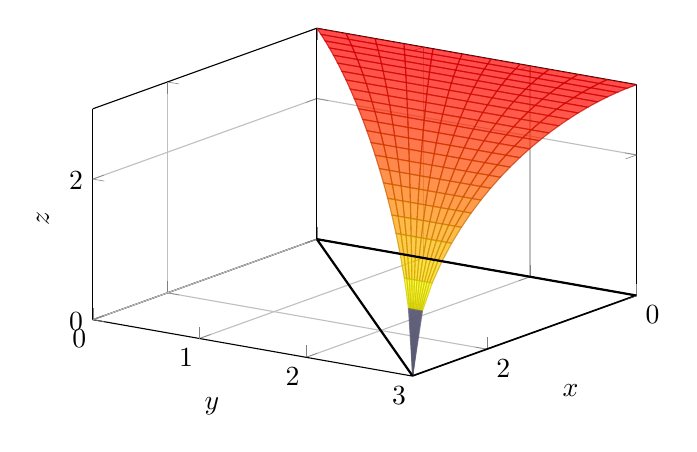
\begin{tikzpicture}\begin{axis}[domain=0:3,y domain=0:1,zmin=0,zmax=3]\addplot3[surf,opacity=.7,samples=24,samples y=12] ({x},{x+(3-x)*y},{sqrt(9-x^2)});\addplot3[black,thick] coordinates {(0,0,0)(0,3,0)(3,3,0)(0,0,0)};\addplot3[black] coordinates {(0,0,0)(0,0,3)};\addplot3[black] coordinates {(0,3,0)(0,3,3)};\end{axis}\end{tikzpicture}\end{center}
\ex{51}
The boundary intersections satisfy $x^3-x=x^2+x$, or $x(x-2)(x+1)=0$. With $x\ge0$ the bounded region is $0\le x\le2$, $x^3-x\le y\le x^2+x$. Consequently
\[V=\int_0^2\int_{x^3-x}^{x^2+x}(x^3y^4+xy^2)dy\,dx
=\int_0^2\left[\frac{x^3y^5}{5}+\frac{xy^3}{3}\right]_{x^3-x}^{x^2+x}dx.\]
Expanding the inner result produces the polynomial
\begin{align*}
G(x)={}&-x^{18}/5+x^{16}-2x^{14}+x^{13}/5+3x^{12}+2x^{11}\\
&+2x^{10}/3+x^9+7x^8/5+x^7/3+x^5+2x^4/3.
\end{align*}
An antiderivative, term by term, is
\begin{align*}
H(x)={}&-x^{19}/95+x^{17}/17-2x^{15}/15+x^{14}/70+3x^{13}/13\\
&+x^{12}/6+2x^{11}/33+x^{10}/10+7x^9/45+x^8/24+x^6/6+2x^5/15.
\end{align*}
Thus $\ans{V=H(2)-H(0)=13984735616/14549535}$. The integrand is nonnegative throughout this region because $x\ge0$ and the powers of $y$ are even, so this signed integral is the volume.
\ex{55}
The given bounds $0\le y\le1$, $0\le x\le y$ describe the triangle above $y=x$ in the unit square, with vertices $(0,0),(0,1),(1,1)$. Vertical slices give $0\le x\le1$, $x\le y\le1$, so
\[\ans{\int_0^1\int_0^yf(x,y)dx\,dy=\int_0^1\int_x^1f(x,y)dy\,dx}.\]
\begin{center}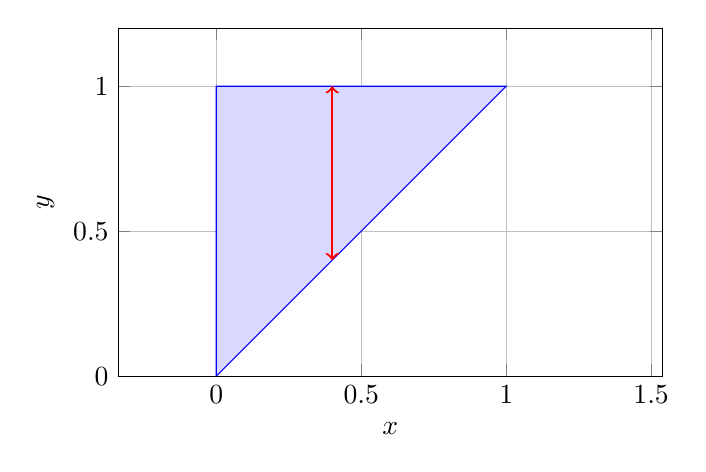
\begin{tikzpicture}\begin{axis}[view={0}{90},axis equal,xmin=0,xmax=1.2,ymin=0,ymax=1.2]\addplot[blue,fill=blue!15] coordinates {(0,0)(0,1)(1,1)(0,0)};\addplot[red,thick,<->] coordinates {(.4,.4)(.4,1)};\end{axis}\end{tikzpicture}\end{center}
\ex{61}
The bounds $0\le y\le1$, $3y\le x\le3$ give the triangle $0\le x\le3$, $0\le y\le x/3$ after reversal. Therefore
\[\int_0^1\int_{3y}^3e^{x^2}dx\,dy=\int_0^3\int_0^{x/3}e^{x^2}dy\,dx
=\frac13\int_0^3xe^{x^2}dx=\ans{(e^9-1)/6}.\]
The original inner antiderivative is not elementary; reversal supplies the factor $x$ needed for $u=x^2$.
\ex{65}
The condition $\arcsin y\le x\le\pi/2$, $0\le y\le1$ is equivalent to $0\le x\le\pi/2$, $0\le y\le\sin x$. Hence
\begin{align*}
I&=\int_0^{\pi/2}\int_0^{\sin x}\cos x\sqrt{1+\cos^2x}\,dy\,dx\\
&=\int_0^{\pi/2}\sin x\cos x\sqrt{1+\cos^2x}\,dx.
\end{align*}
With $u=1+\cos^2x$, $du=-2\sin x\cos x\,dx$, the bounds change from $u=2$ to $u=1$:
\[I=-\tfrac12\int_2^1u^{1/2}du=\tfrac13(2^{3/2}-1)=\ans{(2\sqrt2-1)/3}.\]
\clearpage\section*{15.3 Double Integrals in Polar Coordinates}\addcontentsline{toc}{section}{15.3 Double Integrals in Polar Coordinates}
\noindent Use $x=r\cos\theta$, $y=r\sin\theta$, and $dA=r\,dr\,d\theta$. The additional factor $r$ is the area Jacobian; it is required even when the original integrand is $1$.
\ex{1}
The region is three quarters of the radius-$4$ disk, excluding the fourth quadrant. Polar coordinates give constant bounds:
\[\ans{\iint_R f\,dA=\int_0^{3\pi/2}\int_0^4 f(r\cos\theta,r\sin\theta)r\,dr\,d\theta}.\]
Angles $0$ through $3\pi/2$ sweep the first, second, and third quadrants exactly once.
\ex{2}
The triangle has vertices $(-1,1),(1,1),(1,-1)$. Rectangular coordinates are simpler. At each $-1\le x\le1$, $-x\le y\le1$, so
\[\ans{\iint_R f\,dA=\int_{-1}^1\int_{-x}^1f(x,y)dy\,dx}.\]
The sloping boundary is $y=-x$, and the horizontal boundary is $y=1$.
\ex{3}
The upper half-annulus has inner radius $1$, outer radius $3$, and $y\ge0$. Thus polar coordinates give
\[\ans{\iint_R f\,dA=\int_0^\pi\int_1^3f(r\cos\theta,r\sin\theta)r\,dr\,d\theta}.\]
\ex{4}
The radius-$3$ semicircle lies on the side $x+y\ge0$ of the diagonal diameter. Its rays range from $\theta=-\pi/4$ to $3\pi/4$. Consequently
\[\ans{\iint_R f\,dA=\int_{-\pi/4}^{3\pi/4}\int_0^3f(r\cos\theta,r\sin\theta)r\,dr\,d\theta}.\]
\ex{5}
The triangle has vertices $(-2,0),(0,1),(2,0)$. Rectangular coordinates use two straight-line upper boundaries:
\[\ans{\iint_R f\,dA=\int_{-2}^0\int_0^{1+x/2}f(x,y)dy\,dx
+\int_0^2\int_0^{1-x/2}f(x,y)dy\,dx}.\]
Alternatively, horizontal slices avoid splitting: $\int_0^1\int_{2y-2}^{2-2y}f(x,y)dx\,dy$.
\ex{6}
The full circular ring is $8\le r\le10$. Polar coordinates give
\[\ans{\iint_R f\,dA=\int_0^{2\pi}\int_8^{10}f(r\cos\theta,r\sin\theta)r\,dr\,d\theta}.\]
\ex{7}
The region is an annular sector: $1\le r\le2$, $\pi/4\le\theta\le3\pi/4$. It lies above the origin between rays $y=x$ and $y=-x$, with the two circular arcs as its other boundaries. Its area is
\[A=\int_{\pi/4}^{3\pi/4}\int_1^2r\,dr\,d\theta
=\int_{\pi/4}^{3\pi/4}[r^2/2]_1^2d\theta=\frac32\cdot\frac\pi2=\ans{3\pi/4}.\]
\begin{center}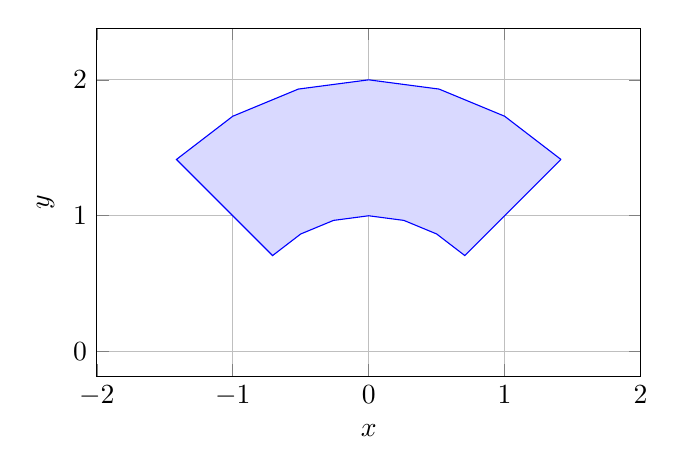
\begin{tikzpicture}\begin{axis}[view={0}{90},axis equal,xmin=-2,xmax=2,ymin=0,ymax=2.2]\addplot[blue,fill=blue!15] coordinates {(1.4142,1.4142)(1,1.7321)(.5176,1.9319)(0,2)(-.5176,1.9319)(-1,1.7321)(-1.4142,1.4142)(-.7071,.7071)(-.5,.8660)(-.2588,.9659)(0,1)(.2588,.9659)(.5,.8660)(.7071,.7071)(1.4142,1.4142)};\end{axis}\end{tikzpicture}\end{center}
\ex{9}
For the top half-disk, $0\le\theta\le\pi$, $0\le r\le5$, and $x^2y=r^3\cos^2\theta\sin\theta$. Thus
\[I=\int_0^\pi\int_0^5r^4\cos^2\theta\sin\theta\,dr\,d\theta
=625\int_0^\pi\cos^2\theta\sin\theta\,d\theta.\]
With $u=\cos\theta$, $du=-\sin\theta d\theta$, the angular integral is $\int_{-1}^1u^2du=2/3$. Therefore $\ans{I=1250/3}$.
\ex{11}
The first-quadrant annulus has $0\le\theta\le\pi/2$, $1\le r\le3$:
\[I=\int_0^{\pi/2}\int_1^3\sin(r^2)r\,dr\,d\theta.
\]
Using $u=r^2$, $du=2rdr$, the radial integral is $[-\cos(r^2)/2]_1^3=(\cos1-\cos9)/2$. Hence
\[\ans{I=\pi(\cos1-\cos9)/4}.\]
\ex{15}
$1\le x^2+y^2\le4$ means $1\le r\le2$, and $0\le y\le x$ means $0\le\theta\le\pi/4$. In this angular interval $\arctan(y/x)=\theta$. Therefore
\[I=\int_0^{\pi/4}\int_1^2\theta r\,dr\,d\theta
=\frac32\int_0^{\pi/4}\theta d\theta=\frac34(\pi/4)^2=\ans{3\pi^2/64}.\]
\ex{17}
The shaded region is inside both cardioids $r=1-\cos\theta$ and $r=1+\cos\theta$. The smaller radius on $0\le\theta\le\pi/2$ is $1-\cos\theta$. Reflection across both axes produces four equal pieces, so
\begin{align*}
A&=4\int_0^{\pi/2}\int_0^{1-\cos\theta}r\,dr\,d\theta
=2\int_0^{\pi/2}(1-\cos\theta)^2d\theta\\
&=2\left[\frac32\theta-2\sin\theta+\frac14\sin2\theta\right]_0^{\pi/2}
=\ans{3\pi/2-4}.
\end{align*}
The antiderivative uses $\cos^2\theta=(1+\cos2\theta)/2$.
\ex{19}
The shaded union of disks $r=\sin\theta$ and $r=\cos\theta$ extends over $-\pi/2\le\theta\le\pi$. The right-hand disk has positive radius for $-\pi/2\le\theta\le\pi/2$; the upper disk for $0\le\theta\le\pi$. On their overlap, the outer boundary changes where $\sin\theta=\cos\theta$, namely $\theta=\pi/4$. Thus the union has radius $\cos\theta$ for $-\pi/2\le\theta\le\pi/4$, and $\sin\theta$ for $\pi/4\le\theta\le\pi$. Its area, counted once, is
\begin{align*}
A&=\frac12\int_{-\pi/2}^{\pi/4}\cos^2\theta d\theta+\frac12\int_{\pi/4}^\pi\sin^2\theta d\theta\\
&=\left[\frac\theta4+\frac{\sin2\theta}{8}\right]_{-\pi/2}^{\pi/4}
+\left[\frac\theta4-\frac{\sin2\theta}{8}\right]_{\pi/4}^\pi
=\ans{3\pi/8+1/4}.
\end{align*}
\ex{21}
The rose petal in the first quadrant begins and ends when $\sin3\theta=0$, at $\theta=0$ and $\pi/3$. In between, the radius is positive. Thus
\[A=\int_0^{\pi/3}\int_0^{\sin3\theta}r\,dr\,d\theta
=\frac12\int_0^{\pi/3}\sin^23\theta d\theta
=\left[\frac\theta4-\frac{\sin6\theta}{24}\right]_0^{\pi/3}=\ans{\pi/12}.\]
\ex{29}
The disk $x^2+y^2\le25$ has $0\le r\le5$. The height is $z=r^2$. Therefore
\[V=\int_0^{2\pi}\int_0^5r^2r\,dr\,d\theta
=2\pi[r^4/4]_0^5=\ans{625\pi/2}.\]
The lower surface is the $xy$ plane; the paraboloid gives the upper surface.
\ex{31}
The plane gives height $z=4-2x-y=4-2r\cos\theta-r\sin\theta$ over $0\le r\le1$, $0\le\theta\le2\pi$. Its height is positive throughout this disk. Thus
\[V=\int_0^{2\pi}\int_0^1(4-2r\cos\theta-r\sin\theta)r\,dr\,d\theta.
\]
The sine and cosine terms integrate to zero over a full revolution; the remaining term gives $V=4(2\pi)(1/2)=\ans{4\pi}$.
\ex{39}
The rectangular bounds describe the first-quadrant quarter-disk $x^2+y^2\le4$. Replace $x^2+y^2$ by $r^2$ and use its polar bounds:
\[I=\int_0^{\pi/2}\int_0^2e^{-r^2}r\,dr\,d\theta
=\frac\pi2[-e^{-r^2}/2]_0^2=\ans{\pi(1-e^{-4})/4}.\]
The substitution $u=-r^2$, $du=-2rdr$ accounts for both the sign and factor $1/2$.
\clearpage\section*{15.4 Applications of Double Integrals}\addcontentsline{toc}{section}{15.4 Applications of Double Integrals}
\noindent For density $\rho$, mass is $m=\iint\rho\,dA$, moments are $M_y=\iint x\rho\,dA$ and $M_x=\iint y\rho\,dA$, and the center of mass is $(\bar x,\bar y)=(M_y/m,M_x/m)$.
\ex{3}
The unit square is darker toward its right side because $\rho=x^2$; therefore estimate $\bar x>1/2$, $\bar y=1/2$. Calculate:
\[m=\int_0^1\int_0^1x^2dy\,dx=\int_0^1x^2dx=1/3,\]
\[M_y=\int_0^1\int_0^1x^3dy\,dx=1/4,\qquad
M_x=\int_0^1x^2[y^2/2]_0^1dx=1/6.\]
Dividing by $m$ gives $\ans{(\bar x,\bar y)=(3/4,1/2)}$, consistent with the shading estimate.
\ex{5}
On $1\le x\le3$, $1\le y\le4$, $\rho=ky^2$, with $k>0$. Thus
\[m=k\int_1^3dx\int_1^4y^2dy=k(2)[y^3/3]_1^4=\ans{42k}.\]
The moments are
\[M_y=k[x^2/2]_1^3[y^3/3]_1^4=k(4)(21)=84k,\]
\[M_x=k\int_1^3dx[y^4/4]_1^4=k(2)(255/4)=255k/2.\]
Therefore $\ans{\bar x=2,\quad\bar y=85/28}$. Uniformity in $x$ places $\bar x$ at the rectangle's midpoint, while the increasing density shifts $\bar y$ above $5/2$.
\ex{7}
For vertices $(0,0),(2,1),(0,3)$, vertical slices are $0\le x\le2$, $x/2\le y\le3-x$. With $\rho=x+y$,
\begin{align*}
m&=\int_0^2[xy+y^2/2]_{x/2}^{3-x}dx
=\int_0^2(9/2-9x^2/8)dx\\
&=[9x/2-3x^3/8]_0^2=9-3=\ans{6},\\
M_y&=\int_0^2[x^2y+xy^2/2]_{x/2}^{3-x}dx
=\int_0^2(9x/2-9x^3/8)dx\\
&=[9x^2/4-9x^4/32]_0^2=9-9/2=9/2,\\
M_x&=\int_0^2[xy^2/2+y^3/3]_{x/2}^{3-x}dx
=\int_0^2(9-9x/2)dx\\
&=[9x-9x^2/4]_0^2=18-9=9.
\end{align*}
Consequently $\ans{(\bar x,\bar y)=(3/4,3/2)}$.
\ex{15}
The lamina is the upper half-annulus $1\le r\le2$, $0\le\theta\le\pi$. Density proportional to distance from the origin means $\rho=kr$, $k>0$. Reflection in the $y$ axis preserves density, so $\bar x=0$ and $M_y=0$. For the other quantities,
\[m=\int_0^\pi\int_1^2(kr)r\,dr\,d\theta
=k\pi[r^3/3]_1^2=7k\pi/3,\]
\[M_x=\int_0^\pi\int_1^2(r\sin\theta)(kr)r\,dr\,d\theta
=k[-\cos\theta]_0^\pi[r^4/4]_1^2=k(2)(15/4)=15k/2.\]
Thus $\ans{(\bar x,\bar y)=(0,45/(14\pi))}$. The proportionality constant cancels in the ratios.
\clearpage\section*{15.5 Surface Area}\addcontentsline{toc}{section}{15.5 Surface Area}
\noindent A graph is parametrized by $r(x,y)=\vv{x,y,f(x,y)}$. Its tangent vectors are $r_x=\vv{1,0,f_x}$ and $r_y=\vv{0,1,f_y}$. The cross product is
\[r_x\times r_y=\cp{1}{0}{f_x}{0}{1}{f_y}
=\ii(0\cdot f_y-f_x\cdot1)-\jj(1\cdot f_y-f_x\cdot0)+\kk(1\cdot1-0\cdot0)
=\vv{-f_x,-f_y,1}.\]
Its length gives $dS=\sqrt{1+f_x^2+f_y^2}\,dx\,dy$. Integrate this over the projection $D$ to obtain area.
\ex{1}
$f=10+x+y^2$ gives $f_x=1$, $f_y=2y$. The figure's projected triangle has vertices $(0,0),(0,-2),(2,-2)$; horizontal slices give $-2\le y\le0$, $0\le x\le-y$. Thus
\[A=\int_{-2}^0\int_0^{-y}\sqrt{2+4y^2}\,dx\,dy
=\int_{-2}^0(-y)\sqrt{2+4y^2}\,dy.\]
With $u=2+4y^2$, $du=8y\,dy$, this becomes
\[A=-\frac18\int_{18}^{2}u^{1/2}du
=\frac{18^{3/2}-2^{3/2}}{12}=\ans{13\sqrt2/3}.\]
\ex{3}
The plane is $z=5x+3y+6$, so $f_x=5$, $f_y=3$ and the area factor is $\sqrt{1+25+9}=\sqrt{35}$. Its rectangle has area $(4-1)(6-2)=12$. Hence $\ans{A=12\sqrt{35}}$.
\ex{5}
For $z=6-3x-2y$, $f_x=-3$, $f_y=-2$, so the area factor is $\sqrt{14}$. In the first octant, the projection is $x,y\ge0$, $3x+2y\le6$, a right triangle with intercepts $2,3$ and area $3$. Thus $\ans{A=3\sqrt{14}}$.
\ex{7}
$z=1-x^2-y^2\ge-2$ gives projection $x^2+y^2\le3$. Since $f_x=-2x$, $f_y=-2y$,
\[A=\int_0^{2\pi}\int_0^{\sqrt3}\sqrt{1+4r^2}r\,dr\,d\theta.
\]
Use $u=1+4r^2$, $du=8rdr$, or the antiderivative $(1+4r^2)^{3/2}/12$:
\[A=\frac{2\pi}{12}[ (1+4r^2)^{3/2}]_0^{\sqrt3}=\ans{\frac\pi6(13\sqrt{13}-1)}.\]
\ex{9}
$z=y^2-x^2$ gives $f_x=-2x$, $f_y=2y$, so the area factor is $\sqrt{1+4r^2}$. Between the cylinders, $1\le r\le2$. Thus
\[A=\int_0^{2\pi}\int_1^2\sqrt{1+4r^2}r\,dr\,d\theta
=\frac\pi6[(1+4r^2)^{3/2}]_1^2=\ans{\frac\pi6(17\sqrt{17}-5\sqrt5)}.\]
\ex{11}
For $z=xy$, $f_x=y$, $f_y=x$. Within $x^2+y^2\le1$, the area is
\[A=\int_0^{2\pi}\int_0^1\sqrt{1+r^2}r\,dr\,d\theta
=\frac{2\pi}{3}[(1+r^2)^{3/2}]_0^1=\ans{\frac{2\pi}{3}(2\sqrt2-1)}.\]
Here $u=1+r^2$, $du=2rdr$, yields $\int r\sqrt{1+r^2}dr=(1+r^2)^{3/2}/3$.
\clearpage\section*{15.6 Triple Integrals}\addcontentsline{toc}{section}{15.6 Triple Integrals}
\ex{3}
\begin{align*}
I&=\int_0^2\int_0^{z^2}\int_0^{y-z}(2x-y)dx\,dy\,dz\\
&=\int_0^2\int_0^{z^2}[x^2-yx]_0^{y-z}dy\,dz
=\int_0^2\int_0^{z^2}(z^2-yz)dy\,dz\\
&=\int_0^2[z^2y-zy^2/2]_0^{z^2}dz
=\int_0^2(z^4-z^5/2)dz\\
&=[z^5/5-z^6/12]_0^2=32/5-16/3=\ans{16/15}.
\end{align*}
These are the given oriented integration bounds; $y-z$ can be negative, so this exercise is a signed iterated integral rather than an everywhere-positive volume calculation.
\ex{5}
\begin{align*}
I&=\int_1^2\int_0^{2z}\int_0^{\ln x}xe^{-y}dy\,dx\,dz\\
&=\int_1^2\int_0^{2z}[-xe^{-y}]_0^{\ln x}dx\,dz
=\int_1^2\int_0^{2z}(x-1)dx\,dz\\
&=\int_1^2[x^2/2-x]_0^{2z}dz=\int_1^2(2z^2-2z)dz\\
&=[2z^3/3-z^2]_1^2=(16/3-4)-(2/3-1)=\ans{5/3}.
\end{align*}
Since $\ln x$ is undefined at $x=0$, the $x$ integration is interpreted as a limit from $x>0$. The integrated expression $x-1$ has a finite limit, so the improper endpoint converges. For $0<x<1$, the inner bounds are reversed and contribute with their stated orientation.
\ex{7}
\begin{align*}
I&=\int_1^3\int_{-1}^2\int_{-y}^z\frac zy dx\,dz\,dy
=\int_1^3\int_{-1}^2\frac zy(z+y)dz\,dy\\
&=\int_1^3\left[\frac{z^3}{3y}+\frac{z^2}{2}\right]_{-1}^2dy
=\int_1^3(3/y+3/2)dy\\
&=[3\ln y+3y/2]_1^3=\ans{3\ln3+3}.
\end{align*}
\ex{9}
\begin{enumerate}[label=(\alph*)]
\item The first-octant figure is bounded by $z=1-x^2$, $y+z=2$, and coordinate planes. Thus $0\le x\le1$, $0\le z\le1-x^2$, and $0\le y\le2-z$:
\[\ans{I=\int_0^1\int_0^{1-x^2}\int_0^{2-z}x\,dy\,dz\,dx}.\]
\item Integrating $y$ gives $x(2-z)$; integrating $z$ gives $x[2z-z^2/2]_0^{1-x^2}=3x/2-x^3-x^5/2$. Therefore $I=[3x^2/4-x^4/4-x^6/12]_0^1=\ans{5/12}$.
\end{enumerate}
\ex{11}
\begin{enumerate}[label=(\alph*)]
\item The figure gives $0\le x\le2$, $0\le y\le x^2$ (the cylinder $x=\sqrt y$), and $0\le z\le2-x$ (the plane $x+z=2$). Hence
\[\ans{I=\int_0^2\int_0^{2-x}\int_0^{x^2}(x+y)dy\,dz\,dx}.\]
\item The inner integral is $[xy+y^2/2]_0^{x^2}=x^3+x^4/2$. Integrating $z$ multiplies by $2-x$, giving $2x^3-x^5/2$. Thus
\[I=[x^4/2-x^6/12]_0^2=8-16/3=\ans{8/3}.\]
\end{enumerate}
\ex{13}
\begin{align*}
I&=\int_0^3\int_0^x\int_{x-y}^{x+y}y\,dz\,dy\,dx
=\int_0^3\int_0^x y[(x+y)-(x-y)]dy\,dx\\
&=\int_0^3\int_0^x2y^2dy\,dx
=\frac23\int_0^3x^3dx=[x^4/6]_0^3=\ans{27/2}.
\end{align*}
The $z$ thickness is $2y$; no other bounds change during the $z$ integration.
\ex{15}
\begin{align*}
I&=\int_0^1\int_0^{y^2}\int_1^{z+1}x^{-3}dx\,dz\,dy\\
&=\frac12\int_0^1\int_0^{y^2}[1-(z+1)^{-2}]dz\,dy\\
&=\frac12\int_0^1[z+(z+1)^{-1}]_0^{y^2}dy
=\frac12\int_0^1\left(y^2+\frac1{1+y^2}-1\right)dy\\
&=\frac12[y^3/3+\arctan y-y]_0^1=\ans{\pi/8-1/3}.
\end{align*}
\ex{17}
The projection is $0\le x\le1$, $0\le y\le\sqrt x$, and $0\le z\le1+x+y$. Therefore
\begin{align*}
I&=\int_0^1\int_0^{\sqrt x}\int_0^{1+x+y}6xy\,dz\,dy\,dx\\
&=\int_0^1\int_0^{\sqrt x}6xy(1+x+y)dy\,dx\\
&=\int_0^1[3x(1+x)y^2+2xy^3]_0^{\sqrt x}dx\\
&=\int_0^1(3x^2+3x^3+2x^{5/2})dx
=1+3/4+4/7=\ans{65/28}.
\end{align*}
\ex{19}
The tetrahedron is $x,y,z\ge0$, $x+y+z\le2$. Use $y$ outermost:
\begin{align*}
I&=\int_0^2\int_0^{2-y}\int_0^{2-y-x}y^2dz\,dx\,dy\\
&=\int_0^2y^2\int_0^{2-y}(2-y-x)dx\,dy
=\frac12\int_0^2y^2(2-y)^2dy\\
&=\frac12[4y^3/3-y^4+y^5/5]_0^2
=\frac12(32/3-16+32/5)=\ans{8/15}.
\end{align*}
\ex{21}
The paraboloid is $x=4(y^2+z^2)$ and the closing plane is $x=4$. Its projection onto the $yz$ plane is the full unit disk. Use polar coordinates in that plane: $y=r\cos\theta$, $z=r\sin\theta$, $dy\,dz=rdrd\theta$. Then
\begin{align*}
I&=\int_0^{2\pi}\int_0^1\int_{4r^2}^4xr\,dx\,dr\,d\theta\\
&=\int_0^{2\pi}\int_0^1\frac r2(16-16r^4)dr\,d\theta
=16\pi\int_0^1(r-r^5)dr\\
&=16\pi(1/2-1/6)=\ans{16\pi/3}.
\end{align*}
\clearpage\section*{15.7 Triple Integrals in Cylindrical Coordinates}\addcontentsline{toc}{section}{15.7 Triple Integrals in Cylindrical Coordinates}
\noindent Cylindrical coordinates use $x=r\cos\theta$, $y=r\sin\theta$, and retain $z$; volume is $dV=r\,dz\,dr\,d\theta$.
\ex{1}
\begin{enumerate}[label=(\alph*)]
\item $(r,\theta,z)=(5,\pi/2,2)$ gives $x=5\cos(\pi/2)=0$, $y=5\sin(\pi/2)=5$, and $z=2$: $\ans{(0,5,2)}$.
\item $(6,-\pi/4,-3)$ gives $x=6/\sqrt2=3\sqrt2$, $y=-6/\sqrt2=-3\sqrt2$, $z=-3$: $\ans{(3\sqrt2,-3\sqrt2,-3)}$.
\end{enumerate}
The plot marks the points and their projections onto the $xy$ plane, so their heights and radial locations are visible.
\begin{center}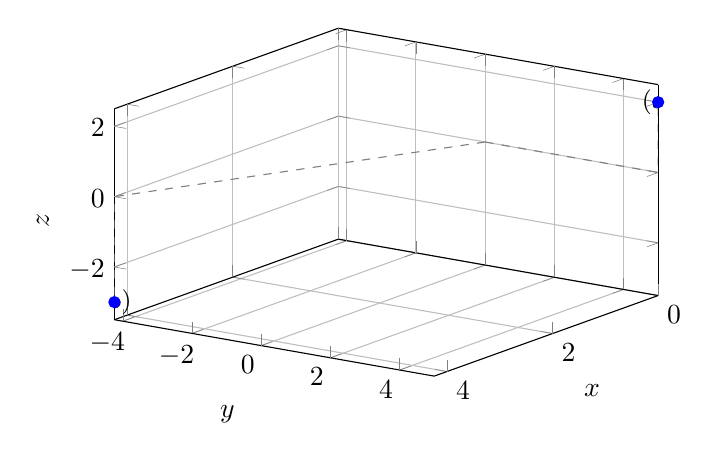
\begin{tikzpicture}\begin{axis}\addplot3[only marks,blue] coordinates {(0,5,2)(4.2426,-4.2426,-3)};\addplot3[gray,dashed] coordinates {(0,0,0)(0,5,0)(0,5,2)};\addplot3[gray,dashed] coordinates {(0,0,0)(4.2426,-4.2426,0)(4.2426,-4.2426,-3)};\node at (axis cs:0,5,2){\small (a)};\node at (axis cs:4.2426,-4.2426,-3){\small (b)};\end{axis}\end{tikzpicture}\end{center}
\ex{3}
\begin{enumerate}[label=(\alph*)]
\item $(4,4,-3)$ has $r=\sqrt{4^2+4^2}=4\sqrt2$ and first-quadrant angle $\theta=\pi/4$. Thus
\[\ans{(r,\theta,z)=(4\sqrt2,\pi/4,-3)}.\]
\item $(5\sqrt3,-5,\sqrt3)$ has $r=\sqrt{75+25}=10$ and fourth-quadrant angle $\theta=-\pi/6$ (equivalently $11\pi/6$), because $\tan\theta=-1/\sqrt3$. Thus $\ans{(10,11\pi/6,\sqrt3)}$.
\end{enumerate}
\ex{5}
$r=2$ means $\sqrt{x^2+y^2}=2$, or $\ans{x^2+y^2=4}$. This is the entire circular cylinder of radius $2$ about the $z$ axis, with arbitrary height and angle. It is a surface, not the solid interior.
\ex{7}
Since $r^2=x^2+y^2$, $r^2+z^2=4$ becomes $\ans{x^2+y^2+z^2=4}$: the sphere centered at the origin with radius $2$.
\ex{9}
\begin{enumerate}[label=(\alph*)]
\item $x^2-x+y^2+z^2=1$ becomes $\ans{r^2-r\cos\theta+z^2=1}$.
\item $z=x^2-y^2$ becomes $r^2(\cos^2\theta-\sin^2\theta)$, so $\ans{z=r^2\cos2\theta}$ by the double-angle identity.
\end{enumerate}
\ex{11}
The inequalities $r^2\le z\le8-r^2$ enclose the region between the upward paraboloid $z=r^2$ and downward paraboloid $z=8-r^2$. They meet when $2r^2=8$, giving $r=2$, $z=4$. Hence the full solid has $0\le r\le2$, $0\le\theta\le2\pi$, with the stated vertical bounds. The two bounding surfaces are shown together:
\begin{center}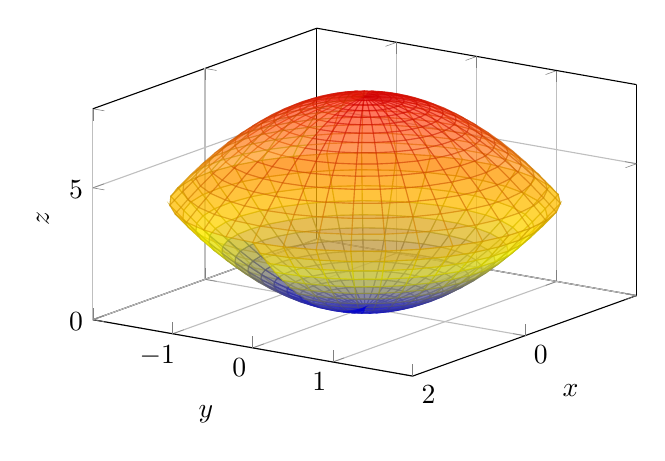
\begin{tikzpicture}\begin{axis}[domain=0:2,y domain=0:360,zmin=0,zmax=8]\addplot3[surf,opacity=.6,samples=16,samples y=36] ({x*cos(y)},{x*sin(y)},{x^2});\addplot3[surf,opacity=.4,samples=16,samples y=36] ({x*cos(y)},{x*sin(y)},{8-x^2});\end{axis}\end{tikzpicture}\end{center}
\ex{15}
\begin{enumerate}[label=(\alph*)]
\item The figure lies inside $r=1$, above $z=0$, and below $z=2-r^2$. The integrand $x^2+y^2$ is $r^2$, so
\[\ans{I=\int_0^{2\pi}\int_0^1\int_0^{2-r^2}r^3\,dz\,dr\,d\theta}.\]
\item Integrate $z$ to obtain $r^3(2-r^2)$, then $r$:
\[I=2\pi[r^4/2-r^6/6]_0^1=2\pi(1/2-1/6)=\ans{2\pi/3}.\]
\end{enumerate}
\ex{17}
The bounds $\pi/2\le\theta\le3\pi/2$, $0\le r\le3$, $r^2\le z\le9$ describe the half of the capped paraboloid solid on the side $x\le0$. Its top is $z=9$, its lower surface is $z=x^2+y^2$, and its flat cut face is in $x=0$. Its volume is
\[V=\int_{\pi/2}^{3\pi/2}\int_0^3\int_{r^2}^9r\,dz\,dr\,d\theta
=\pi\int_0^3(9r-r^3)dr
=\pi[9r^2/2-r^4/4]_0^3=\ans{81\pi/4}.\]
\begin{center}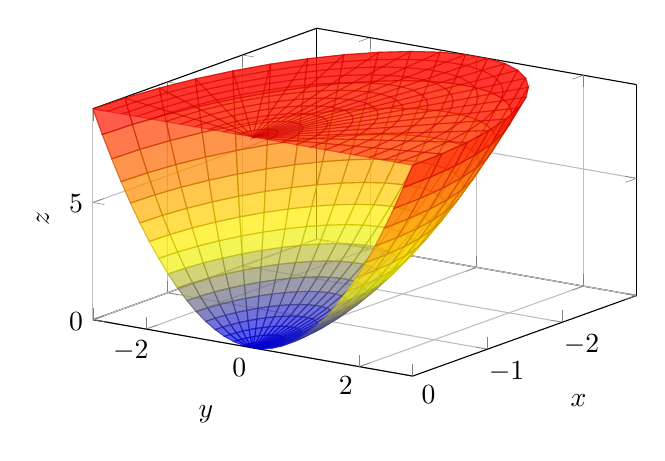
\begin{tikzpicture}\begin{axis}[domain=0:3,y domain=90:270,zmin=0,zmax=9]\addplot3[surf,opacity=.7,samples=18,samples y=24] ({x*cos(y)},{x*sin(y)},{x^2});\addplot3[surf,opacity=.4,samples=12,samples y=24] ({x*cos(y)},{x*sin(y)},{9});\end{axis}\end{tikzpicture}\end{center}
\ex{21}
In the first octant, $0\le\theta\le\pi/2$, $0\le r\le2$, $0\le z\le4-r^2$. Thus
\begin{align*}
I&=\int_0^{\pi/2}\int_0^2\int_0^{4-r^2}(r\cos\theta+r\sin\theta+z)r\,dz\,dr\,d\theta\\
&=\int_0^{\pi/2}\int_0^2\left[r^2(\cos\theta+\sin\theta)(4-r^2)+\frac r2(4-r^2)^2\right]dr\,d\theta.
\end{align*}
The angular integrals are $\int_0^{\pi/2}(\cos\theta+\sin\theta)d\theta=2$ and $\int_0^{\pi/2}d\theta=\pi/2$. Hence
\[I=2[4r^3/3-r^5/5]_0^2+\frac\pi4[8r^2-2r^4+r^6/6]_0^2
=\ans{128/15+8\pi/3}.\]
\ex{23}
Inside the cylinder $r\le1$ and below the upper cone $z=2r$, with $z\ge0$, the integrand $x^2=r^2\cos^2\theta$. Therefore
\[I=\int_0^{2\pi}\int_0^1\int_0^{2r}r^3\cos^2\theta\,dz\,dr\,d\theta
=2\int_0^{2\pi}\cos^2\theta d\theta\int_0^1r^4dr=2(\pi)(1/5)=\ans{2\pi/5}.\]
Here the condition $z\ge0$ selects the positive branch of the cone equation $z^2=4r^2$.
\ex{29}
The constant-density solid has $4r^2\le z\le a$, so $0\le r\le\sqrt a/2$, $0\le\theta\le2\pi$. Symmetry gives $\bar x=\bar y=0$. With density $K$,
\[m=2\pi K\int_0^{\sqrt a/2}(a-4r^2)rdr
=2\pi K[ar^2/2-r^4]_0^{\sqrt a/2}=\ans{K\pi a^2/8}.\]
For the vertical moment,
\[M_{xy}=2\pi K\int_0^{\sqrt a/2}[z^2/2]_{4r^2}^a r\,dr
=\pi K[a^2r^2/2-8r^6/3]_0^{\sqrt a/2}=K\pi a^3/12.\]
Thus $\ans{(\bar x,\bar y,\bar z)=(0,0,2a/3)}$.
\ex{30}
Density proportional to distance from the $z$ axis means $\rho=kr$, $k>0$. In the ball, $0\le r\le a$, $-\sqrt{a^2-r^2}\le z\le\sqrt{a^2-r^2}$, so
\[m=\int_0^{2\pi}\int_0^a\int_{-\sqrt{a^2-r^2}}^{\sqrt{a^2-r^2}}kr^2dz\,dr\,d\theta
=4\pi k\int_0^ar^2\sqrt{a^2-r^2}dr.\]
Let $r=a\sin u$, $dr=a\cos u\,du$, $0\le u\le\pi/2$. Then
\[m=4\pi ka^4\int_0^{\pi/2}\sin^2u\cos^2u\,du
=\frac{\pi ka^4}{2}\int_0^{\pi/2}(1-\cos4u)du=\ans{\pi^2ka^4/4}.\]
The identity $\sin^2u\cos^2u=(1-\cos4u)/8$ produces the last step.
\clearpage\section*{15.8: Spherical coordinates}\addcontentsline{toc}{section}{15.8: Spherical coordinates}
Throughout this section, $x=\rho\sin\phi\cos\theta$, $y=\rho\sin\phi\sin\theta$, $z=\rho\cos\phi$, and $dV=\rho^2\sin\phi\,d\rho\,d\phi\,d\theta$. The angle $\phi$ is measured down from the positive $z$ axis; $\theta$ is measured in the $xy$ plane from positive $x$ toward positive $y$.
\ex{1}
\textbf{(a)} For $(\rho,\theta,\phi)=(2,3\pi/4,\pi/2)$,
\[x=2(1)(-\sqrt2/2)=-\sqrt2,\quad y=2(1)(\sqrt2/2)=\sqrt2,\quad z=2(0)=0.\]
Thus the point is $\ans{(-\sqrt2,\sqrt2,0)}$, in quadrant II of the $xy$ plane.
\textbf{(b)} For $(4,-\pi/3,\pi/4)$,
\[x=4(\sqrt2/2)(1/2)=\sqrt2,\quad y=4(\sqrt2/2)(-\sqrt3/2)=-\sqrt6,\quad z=4\sqrt2/2=2\sqrt2.\]
The point is $\ans{(\sqrt2,-\sqrt6,2\sqrt2)}$, above quadrant IV.
\begin{center}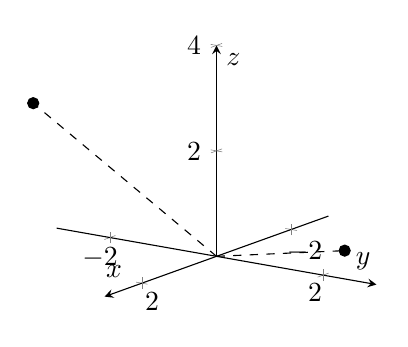
\begin{tikzpicture}\begin{axis}[axis lines=center,xmin=-3,xmax=3,ymin=-3,ymax=3,zmin=0,zmax=4]
\addplot3[only marks,mark=*] coordinates {(-1.414,1.414,0) (1.414,-2.449,2.828)};
\addplot3[dashed] coordinates {(0,0,0) (-1.414,1.414,0)};
\addplot3[dashed] coordinates {(0,0,0) (1.414,-2.449,2.828)};
\end{axis}\end{tikzpicture}\end{center}
\ex{3}
\textbf{(a)} For $(3,3,0)$, $\rho=\sqrt{9+9}=3\sqrt2$, $\tan\theta=1$ in quadrant I gives $\theta=\pi/4$, and $\cos\phi=z/\rho=0$ gives $\phi=\pi/2$. Hence $\ans{(3\sqrt2,\pi/4,\pi/2)}$.
\textbf{(b)} For $(1,-\sqrt3,2\sqrt3)$,
\[\rho=\sqrt{1+3+12}=4,\quad \theta=5\pi/3,\quad \cos\phi=2\sqrt3/4=\sqrt3/2.\]
Quadrant IV determines $\theta$; the positive height determines $\phi=\pi/6$. Therefore $\ans{(4,5\pi/3,\pi/6)}$.
\ex{5}
The fixed angle $\phi=3\pi/4$ describes the downward half of a circular cone, with vertex at the origin and axis the $z$ axis. Since $r=\rho\sin\phi=\rho/\sqrt2$ and $z=\rho\cos\phi=-\rho/\sqrt2$, its rectangular equation is $\ans{z=-\sqrt{x^2+y^2}}$.
\ex{7}
Since $z=\rho\cos\phi$, the equation is $\ans{z=1}$: a horizontal plane one unit above the $xy$ plane.
\ex{9}
\textbf{(a)} $x^2+y^2+z^2=\rho^2$, so $\rho^2=9$. With $\rho\ge0$, $\ans{\rho=3}$.
\textbf{(b)} Direct substitution gives
\[\rho^2\sin^2\phi\cos^2\theta-\rho^2\sin^2\phi\sin^2\theta-\rho^2\cos^2\phi=1.\]
Using $\cos^2\theta-\sin^2\theta=\cos2\theta$, this becomes $\ans{\rho^2(\sin^2\phi\cos2\theta-\cos^2\phi)=1}$.
\ex{11}
The solid is inside the unit sphere, above the cone $z=\sqrt3\sqrt{x^2+y^2}$, and on the $y\ge0$ side. Indeed $\phi\le\pi/6$ gives $z/r\ge\cot(\pi/6)=\sqrt3$, while $0\le\theta\le\pi$ gives $y\ge0$. It is half of a narrow spherical sector about the positive $z$ axis.
\surf{domain=0:180,y domain=0:30}{sin(y)*cos(x)}{sin(y)*sin(x)}{cos(y)}
\ex{13}
The bounds $1\le\rho\le3$ select a spherical shell; $0\le\phi\le\pi/2$ selects the upper half; $\pi\le\theta\le3\pi/2$ selects quadrant III. Thus this is the upper part of the shell with $x\le0$, $y\le0$, $z\ge0$.
\begin{center}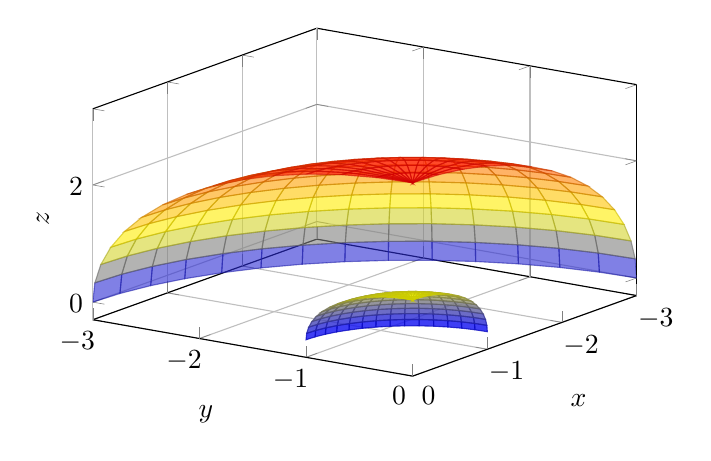
\begin{tikzpicture}\begin{axis}
\addplot3[surf,opacity=.6,domain=180:270,y domain=0:90,samples=15] ({3*sin(y)*cos(x)},{3*sin(y)*sin(x)},{3*cos(y)});
\addplot3[surf,opacity=.8,domain=180:270,y domain=0:90,samples=15] ({sin(y)*cos(x)},{sin(y)*sin(x)},{cos(y)});
\end{axis}\end{tikzpicture}\end{center}
\ex{15}
The sphere gives $0\le\rho\le2$. The cone $z=r$ corresponds to $\phi=\pi/4$. Outside the upward cone means below its surface, so
\[\ans{0\le\rho\le2,\quad \pi/4\le\phi\le\pi,\quad0\le\theta\le2\pi}.\]
The lower hemisphere is included: it is entirely outside this upward cone.
\ex{17}
The bounds describe a radius-3 spherical sector with $0\le\theta\le\pi/2$ and $0\le\phi\le\pi/6$: the first-quadrant half of the sector above $z=\sqrt3r$.
\[V=\int_0^{\pi/6}\int_0^{\pi/2}\int_0^3\rho^2\sin\phi\,d\rho\,d\theta\,d\phi
=9\frac\pi2[-\cos\phi]_0^{\pi/6}=\ans{\frac{9\pi}{4}(2-\sqrt3)}.\]
\surf{domain=0:90,y domain=0:30}{3*sin(y)*cos(x)}{3*sin(y)*sin(x)}{3*cos(y)}
\ex{21}
\textbf{(a)} The pictured region is the lower half of the shell between radii 2 and 3. The integrand becomes $f=\rho$, hence
\[I=\int_0^{2\pi}\int_{\pi/2}^{\pi}\int_2^3\rho^3\sin\phi\,d\rho\,d\phi\,d\theta.\]
\textbf{(b)} Integrating each factor,
\[I=(2\pi)[-\cos\phi]_{\pi/2}^{\pi}[\rho^4/4]_2^3
=2\pi(1)\frac{81-16}{4}=\ans{65\pi/2}.\]
\ex{23}
The integrand is $(\rho^2)^2=\rho^4$, and the ball has $0\le\rho\le5$:
\[I=\int_0^{2\pi}\int_0^\pi\int_0^5\rho^6\sin\phi\,d\rho\,d\phi\,d\theta
=2\pi(2)[\rho^7/7]_0^5=\ans{312500\pi/7}.\]
\ex{25}
Since $x^2+y^2=\rho^2\sin^2\phi$,
\[I=\int_0^{2\pi}\int_0^\pi\int_2^3\rho^4\sin^3\phi\,d\rho\,d\phi\,d\theta.\]
With $u=\cos\phi$,
\[\int_0^\pi\sin^3\phi\,d\phi=\int_{-1}^1(1-u^2)du=[u-u^3/3]_{-1}^1=4/3.\]
Therefore $I=2\pi(4/3)(243-32)/5=\ans{1688\pi/15}$.
\ex{27}
The first octant gives $0\le\theta,\phi\le\pi/2$. Substituting both the function and volume factor,
\[I=\int_0^{\pi/2}\int_0^{\pi/2}\int_0^1\rho^3e^{\rho^2}\sin^2\phi\cos\theta\,d\rho\,d\phi\,d\theta.\]
The $\theta$ factor is $[\sin\theta]_0^{\pi/2}=1$; the $\phi$ factor is $\int_0^{\pi/2}(1-\cos2\phi)/2\,d\phi=\pi/4$. Set $u=\rho^2$, so $\rho^3d\rho=u\,du/2$. Integration by parts gives
\[\int_0^1\rho^3e^{\rho^2}d\rho=\frac12\int_0^1ue^udu
=\frac12[(u-1)e^u]_0^1=1/2.\]
Thus $\ans{I=\pi/8}$.
\ex{41}
Cylindrical coordinates simplify the boundaries. The paraboloid is $z=r^2$ and the plane is $z=2r\sin\theta$. Their intersection gives $r=2\sin\theta$, with $0\le\theta\le\pi$. Therefore
\begin{align*}
I&=\int_0^\pi\int_0^{2\sin\theta}\int_{r^2}^{2r\sin\theta}zr\,dz\,dr\,d\theta\\
&=\frac12\int_0^\pi\int_0^{2\sin\theta}(4r^3\sin^2\theta-r^5)dr\,d\theta\\
&=\frac12\int_0^\pi[r^4\sin^2\theta-r^6/6]_0^{2\sin\theta}d\theta
=\frac83\int_0^\pi\sin^6\theta\,d\theta.
\end{align*}
The reduction formula $J_n=(n-1)J_{n-2}/n$, $J_0=\pi$, gives $J_6=(5/6)(3/4)(1/2)\pi=5\pi/16$. Hence $\ans{I=5\pi/6}$.
\ex{43}
The $xy$ projection is a quarter unit disk. The lower surface is the cone $z=r$ and the upper surface is the sphere $\rho=\sqrt2$. Consequently $0\le\theta\le\pi/2$, $0\le\phi\le\pi/4$, and $0\le\rho\le\sqrt2$. Since $xy=\rho^2\sin^2\phi\cos\theta\sin\theta$,
\[I=\int_0^{\pi/2}\int_0^{\pi/4}\int_0^{\sqrt2}\rho^4\sin^3\phi\cos\theta\sin\theta\,d\rho\,d\phi\,d\theta.\]
The three factors are respectively $1/2$, $[-\cos\phi+\cos^3\phi/3]_0^{\pi/4}=2/3-5\sqrt2/12$, and $[\rho^5/5]_0^{\sqrt2}=4\sqrt2/5$. Thus
\[I=\frac12\left(\frac23-\frac{5\sqrt2}{12}\right)\frac{4\sqrt2}{5}=\ans{\frac{4\sqrt2-5}{15}}.\]
\ex{48}
Let latitude be $\alpha$ and west longitude be $\beta$. A unit position vector is
\[\mathbf u=(\cos\alpha\cos\beta,-\cos\alpha\sin\beta,\sin\alpha).\]
The minus sign accounts for west longitude. The central angle $\gamma$ between two locations satisfies
\[\cos\gamma=\mathbf u_1\cdot\mathbf u_2
=\sin\alpha_1\sin\alpha_2+\cos\alpha_1\cos\alpha_2\cos(\beta_1-\beta_2).\]
For the given coordinates, $\alpha_1=34.06^\circ$, $\alpha_2=45.50^\circ$, and $\beta_1-\beta_2=118.25^\circ-73.60^\circ=44.65^\circ$. Thus
\[\cos\gamma\approx0.8125593358,\quad \gamma\approx0.6222666978\text{ radians}.\]
The great-circle arc length is radius times central angle in radians:
\[d=3960\gamma\approx\ans{2464\text{ miles}}.\]

\clearpage\section*{15.9: Changes of variables}\addcontentsline{toc}{section}{15.9: Changes of variables}
For $x=x(u,v)$ and $y=y(u,v)$, the area factor is the absolute value of the Jacobian $J=x_uy_v-x_vy_u$. Transform the boundary as well as the integrand; a determinant by itself does not determine the new limits.
\ex{1}
\textbf{(a)} The four corners map to $(0,0),(1,1),(1,-1),(2,0)$, so the image is the diamond \textbf{VI}.
\textbf{(b)} $x=u-v$ and $y=uv$. On $v=0$ and $u=0$, $y=0$, with $-1\le x\le1$. On $u=1$, $y=v=1-x$; on $v=1$, $y=u=x+1$. Thus the triangle is \textbf{I}.
\textbf{(c)} $x=u\cos v$, $y=u\sin v$ are polar coordinates with radius $0\le u\le1$ and angle $0\le v\le1$ radian. This is sector \textbf{IV}.
\textbf{(d)} On $u=0$, $(x,y)=(-v,v^2)$, giving $y=x^2$ on $-1\le x\le0$. On $u=1$, $(x,y)=(1-v,1+v^2)$, giving $y=1+(1-x)^2$ on $0\le x\le1$. The other sides, $v=0$ and $v=1$, are $y=x$ and $y=x+2$. These curved sides identify \textbf{V}.
\textbf{(e)} The corners map to $(0,0),(1,0),(1,2),(2,2)$. The image is parallelogram \textbf{III}.
\textbf{(f)} Both axes $u=0$ and $v=0$ map to $x=0$, with $-1\le y\le1$. The sides $u=1$ and $v=1$ become $y=1-x^3$ and $y=x^3-1$, $0\le x\le1$. Thus the rightward curved region is \textbf{II}.
\ex{3}
For $x=2u+3v$, $y=u-v$, transform the rectangle's corners in order:
\[(0,0)\mapsto(0,0),\quad(3,0)\mapsto(6,3),\]
\[(3,2)\mapsto(12,1),\quad(0,2)\mapsto(6,-2).\]
The image is a parallelogram.
Solving the equations gives $u=(x+3y)/5$, $v=(x-2y)/5$. Therefore the full image is
\[\ans{0\le x+3y\le15,\qquad0\le x-2y\le10}.\]
\begin{center}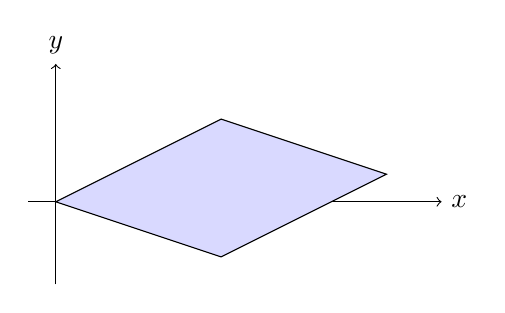
\begin{tikzpicture}[scale=.35]\draw[->] (-1,0)--(14,0) node[right]{$x$};\draw[->] (0,-3)--(0,5) node[above]{$y$};\draw[fill=blue!15] (0,0)--(6,3)--(12,1)--(6,-2)--cycle;\end{tikzpicture}\end{center}
\ex{5}
The original triangle has $u\ge0$, $v\ge0$, $u+v\le1$. Since $x=u^2$ is increasing for $u\ge0$, $u=\sqrt x$; $v=y$. Thus
\[\ans{0\le x\le1,\quad0\le y\le1-\sqrt x}.\]
The coordinate-axis sides remain on the axes, while the sloping side becomes $y=1-\sqrt x$.
\begin{center}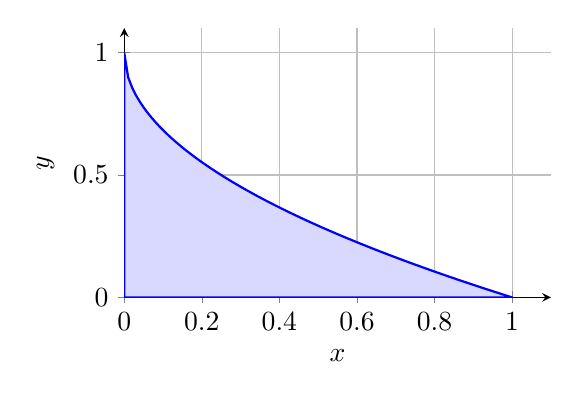
\begin{tikzpicture}\begin{axis}[width=7cm,height=5cm,axis lines=left,xlabel=$x$,ylabel=$y$,xmin=0,xmax=1.1,ymin=0,ymax=1.1]
\addplot[blue,thick,domain=0:1,samples=100,fill=blue!15] {1-sqrt(x)}\closedcycle;
\end{axis}\end{tikzpicture}\end{center}
\ex{6}
Assuming the usual positive scale constants $a,b$, $u=x/a$, $v=y/b$, so the unit disk maps to
\[\ans{x^2/a^2+y^2/b^2\le1}.\]
This is the filled ellipse centered at the origin with semiaxes $a$ and $b$ along the coordinate axes. The same equation applies for nonzero negative scale constants, with semiaxis lengths $|a|,|b|$.
\ex{7}
Choose $u=y-2x$, $v=x+y$. The four boundaries become $u=-1$, $u=1$, $v=1$, $v=3$, so $S=[-1,1]\times[1,3]$. Adding $v$ to $-u$ gives $3x=v-u$; then $y=v-x$. Hence
\[\ans{x=(v-u)/3,\qquad y=(2v+u)/3}.\]
This invertible linear transformation maps the rectangle exactly onto the given parallelogram.
\ex{11}
\[J=\begin{vmatrix}2&1\\4&-1\end{vmatrix}=2(-1)-1(4)=\ans{-6}.\]
The Jacobian is signed; an integral uses $|J|=6$.
\ex{13}
For $x=s\cos t$, $y=s\sin t$,
\[J=\begin{vmatrix}\cos t&-s\sin t\\\sin t&s\cos t\end{vmatrix}
=s\cos^2t+s\sin^2t=\ans{s}.\]
\ex{15}
For $x=uv$, $y=vw$, $z=wu$, expand along the first row:
\begin{align*}
J&=\begin{vmatrix}v&u&0\\0&w&v\\w&0&u\end{vmatrix}\\
&=v\begin{vmatrix}w&v\\0&u\end{vmatrix}-u\begin{vmatrix}0&v\\w&u\end{vmatrix}
=v(wu-0)-u(0-vw)=\ans{2uvw}.
\end{align*}
\ex{23}
\textbf{(a)} Under $x=au$, $y=bv$, $z=cw$, the ellipsoid becomes the unit ball $u^2+v^2+w^2\le1$. For positive semiaxes,
\[J=\begin{vmatrix}a&0&0\\0&b&0\\0&0&c\end{vmatrix}=a(bc-0)=abc.\]
Consequently
\[V=abc\int_0^{2\pi}\int_0^\pi\int_0^1\rho^2\sin\phi\,d\rho\,d\phi\,d\theta
=abc(2\pi)(2)(1/3)=\ans{4\pi abc/3}.\]
\textbf{(b)} Substituting the supplied equatorial and polar radii gives
\[V=\frac{4\pi}{3}(6378)^2(6356)\approx\ans{1.08303\times10^{12}\text{ km}^3}.\]
\textbf{(c)} For constant density $k$,
\[I_z=\iiint_E(x^2+y^2)k\,dV=kabc\iiint_B(a^2u^2+b^2v^2)dV.\]
Rotational symmetry gives equal integrals of $u^2,v^2,w^2$. Their sum is
\[\iiint_B(u^2+v^2+w^2)dV=4\pi\int_0^1\rho^4d\rho=4\pi/5,\]
so each is $4\pi/15$. Therefore
\[\ans{I_z=4\pi kabc(a^2+b^2)/15=\frac{M}{5}(a^2+b^2)},\quad M=4\pi kabc/3.\]
\ex{25}
Choose $u=x-2y$, $v=3x-y$; the region becomes $0\le u\le4$, $1\le v\le8$, and the integrand becomes $u/v$. Solving gives $y=(v-3u)/5$, $x=(2v-u)/5$. Thus
\[J=\begin{vmatrix}-1/5&2/5\\-3/5&1/5\end{vmatrix}=-1/25+6/25=1/5.\]
The transformed integral is
\[I=\frac15\int_1^8\int_0^4\frac uv\,du\,dv
=\frac15\int_1^8\frac8v\,dv=\ans{\frac85\ln8=\frac{24}{5}\ln2}.\]

\end{document}
